\documentclass[
    11pt,
    spanish,
	a4paper
]{article}
\usepackage[utf8]{inputenc}
\usepackage[spanish]{babel}
\usepackage{graphicx}
\usepackage{authoraftertitle}
\usepackage{float}
\usepackage{caption}
\usepackage{verbatim}
\captionsetup[table]{labelformat=empty}

\def\doctype{INFORME DE INVESTIGACIÓN}
\title{Softwares de Simulación para Tecnología Electrónica y otras cátedras de
  Ingeniera.}
\author{Gonzalo Nahuel Vaca}

\begin{document}

\makeatletter
\begin{titlepage}
	\begin{center}
		\vspace*{1cm}
		
		\Huge
		\textbf{\doctype}
		\vspace{0.5cm}
    
		\LARGE
		\@title
		\vspace{0.5cm}
    
		\textbf{Compatibilidad Electromagnética}
		
		\vspace{1.5cm}
		
		\textbf{\@author}

		\vspace{3.5cm}

		%
\includegraphics[width=0.8\textwidth]{img/logoFIUBA.pdf}
		
		\vfill
		Departamento de Ingeniería e Investigaciones Tecnológicas\\
		Universidad Nacional de la Matanza\\
		Argentina\\
		\today
	\end{center}
\end{titlepage}
\makeatother
\newpage

\section{Introducción}
\label{sec:introduccion}

Este documento se propone detallar todos los aspectos referidos a la evaluación
de programas para el cálculo de compatibilidad electromagnética.

\section{OpenEMS}
\label{sec:openems}

En esta sección se encuentran los detalles de la evaluación del programa OpenEMS.

\subsection{Instalación}
\label{sub:oinstalacion}

A continuación se detallan los pasos a seguir para tener el programa instalado
en el ordenador.

\begin{enumerate}
  \item Satisfacer las dependencias del programa, a continuación se muestran los
    comandos para el sistema Ubuntu 22.04 LTS:
    \begin{itemize}
      \item Dependencias mínimas obligatorias:\\
        \texttt{sudo apt-get install\\
        build-essential cmake git libhdf5-dev libvtk7-dev\\
        libboost-all-dev libcgal-dev libtinyxml-dev\\
        qtbase5-dev libvtk7-qt-dev}
      \item GNU Octave (equivalente GNU de Matlab, opcional):\\
        \texttt{sudo apt-get install octave liboctave-dev}
      \item Interfaz Python (opcional):\\
        \texttt{sudo pip3 install matplotlib cython h5py}
    \end{itemize}
  \item Clonar e instalar
    \begin{itemize}
      \item Clonar el repositorio y sus submódulos:\\
        \texttt{git clone --recursive\\
          https://github.com/thliebig/openEMS-Project.git}
      \item Dentro del repositorio ejecutar:
        \begin{verbatim}
./update_openEMS.sh ~/opt/openEMS --python
        \end{verbatim}
    \end{itemize}
\end{enumerate}

\subsection{Verificación}
\label{sub:overificacion}

La prueba más simple para verificar la instalación es ejecutar el binario de
openEMS.
Para lograrlo debe navegar hasta la carpeta de la instalación, la cuál
normalmente es \texttt{opt/openEMS/bin} dentro de su usuario; luego se debe ejecutar
el comando \texttt{./openEMS} y deberá observar una salida como la siguiente:

\begin{verbatim}
--------------------------------------------------------
| openEMS 64bit -- version v0.0.35-76-gd4448fa
| (C) 2010-2018 Thorsten Liebig <thorsten.liebig@gmx.de>
| GPL license
--------------------------------------------------------
Used external libraries:
CSXCAD -- Version: v0.6.2-109-gcd9decb
hdf5   -- Version: 1.10.7
compiled against: HDF5 library version: 1.10.7
tinyxml -- compiled against: 2.6.2
fparser
boost  -- compiled against: 1_74
vtk -- Version: 7.1.1
compiled against: 7.1.1
\end{verbatim}

A continuación se detallan los pasos a seguir para verificar la correcta
instalación de openEMS con GNU Octave.

Como se muestra en la figura \ref{fig:octavepath} se debe colocar el \emph{path}
de openEMS en la ventana de comandos.

Los comandos para agregar los \emph{path} son:

\begin{verbatim}
addpath('~/opt/openEMS/share/openEMS/matlab');
addpath('~/opt/openEMS/share/CSXCAD/matlab');
\end{verbatim}

\begin{figure}[htbp]
	\centering
	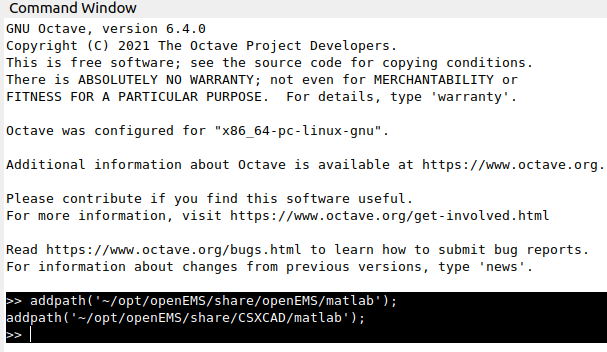
\includegraphics[width=\textwidth]{./img/octavepath.png}
	\caption{Configuración de \emph{path} en GNU Octave.}
	\label{fig:octavepath}
\end{figure}

El siguiente paso es verificar la interfaz CXCAD, a continuación se muestra el
comando y respuesta en la ventana de comandos de GNU Octave:

\begin{verbatim}
>> InitCSX
ans = 
Properties: []
\end{verbatim}

Con la interfaz inicializada se puede realizar una verificación de sus funciones
como se muestra a continuación:

\begin{verbatim}
>> InitFDTD('NrTS', 0, 'EndCriteria', 0)
ans = 
    ATTRIBUTE: [1x1 struct]
\end{verbatim}

El siguiente paso es verificar el correcto funcionamiento del simulador como se
muestra a continuación:

\begin{verbatim}
>> RunOpenEMS( '.', 'nonexistant.xml', '' )
[...]
Read openEMS xml file: nonexistant.xml ...
openEMS: Error File-Loading failed!!! File: nonexistant.xml
\end{verbatim}

El error que se muestra significa que el simulador funciona correctamente ya que
su argumento es un archivo inexistente. Sin embargo, el binario del simulador se
invocó sin problemas.

Es importante verificar que el programa de visualización de definiciones de
geometría funcione de forma correcta, esto se logra con el siguiente comando:

\begin{verbatim}
CSXGeomPlot('nonexistant.xml')
\end{verbatim}

La ventana de comandos debe arrojar un error ya que el archivo de geometría no
existe, sin embargo se debe ejecutar el visualizador como se muestra en la
figura \ref{fig:geovisual}.

Llegado a este punto se puede concluir que openEMS fue instalado de forma correcta.

\begin{figure}[htbp]
	\centering
	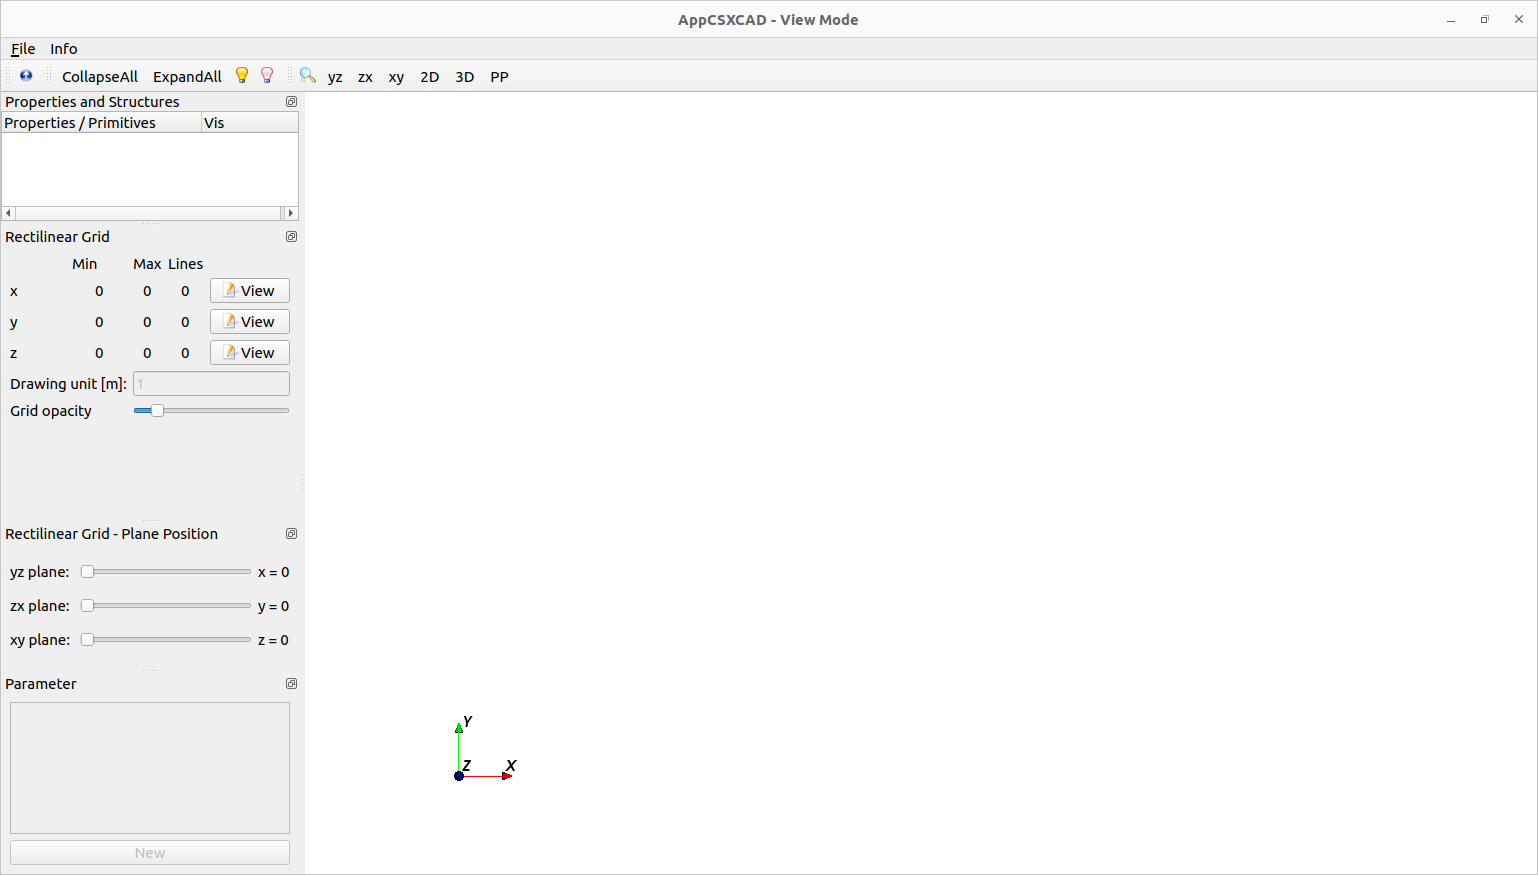
\includegraphics[width=\textwidth]{./img/geovisual.png}
	\caption{Programa de visualización de geometrías.}
	\label{fig:geovisual}
\end{figure}

Se recomienda instalar el programa ParaView para tener una herramienta para
visualizar las simulaciones.
Los ejemplos de este documento utilizan ParaView para representar de forma
gráfica los resultados.

\subsection{Ejemplos de uso}
\label{sub:oejemplos}

\subsubsection{Guía de onda superficial}
\label{subsub:oejemplo1}

Las instrucciones para generar la geometría, su excitación y la definición de
las variables a observar son las siguientes:

\begin{verbatim}
close all
clear
clc
FDTD = InitFDTD('NrTS',100, 'EndCriteria',0, 'OverSampling',50);
FDTD = SetSinusExcite(FDTD,10e6);
FDTD = SetBoundaryCond(FDTD,{'PMC' 'PMC' 'PEC' 'PEC' 'MUR' 'MUR'});
CSX = InitCSX();
mesh.x = -10:10;
mesh.y = -10:10;
mesh.z = -10:30;
CSX = DefineRectGrid(CSX, 1, mesh);
CSX = AddExcitation(CSX,'excitation',0,[0 1 0]);
CSX = AddBox(CSX,'excitation',0,[-10 -10 0],[10 10 0]);
CSX = AddDump(CSX,'Et');
CSX = AddBox(CSX,'Et',0,[-10 0 -10],[10 0 30]);
mkdir('tmp');
WriteOpenEMS('tmp/tmp.xml',FDTD,CSX);
\end{verbatim}

Antes de lanzar la simulación se procede a verificar la geometría generada con
los siguientes comandos:

\begin{verbatim}
CSXGeomPlot( 'tmp/tmp.xml' );
\end{verbatim}

En la figura \ref{fig:geo1} se puede observar el plano que simula una guía de onda.

\begin{figure}[htbp]
	\centering
	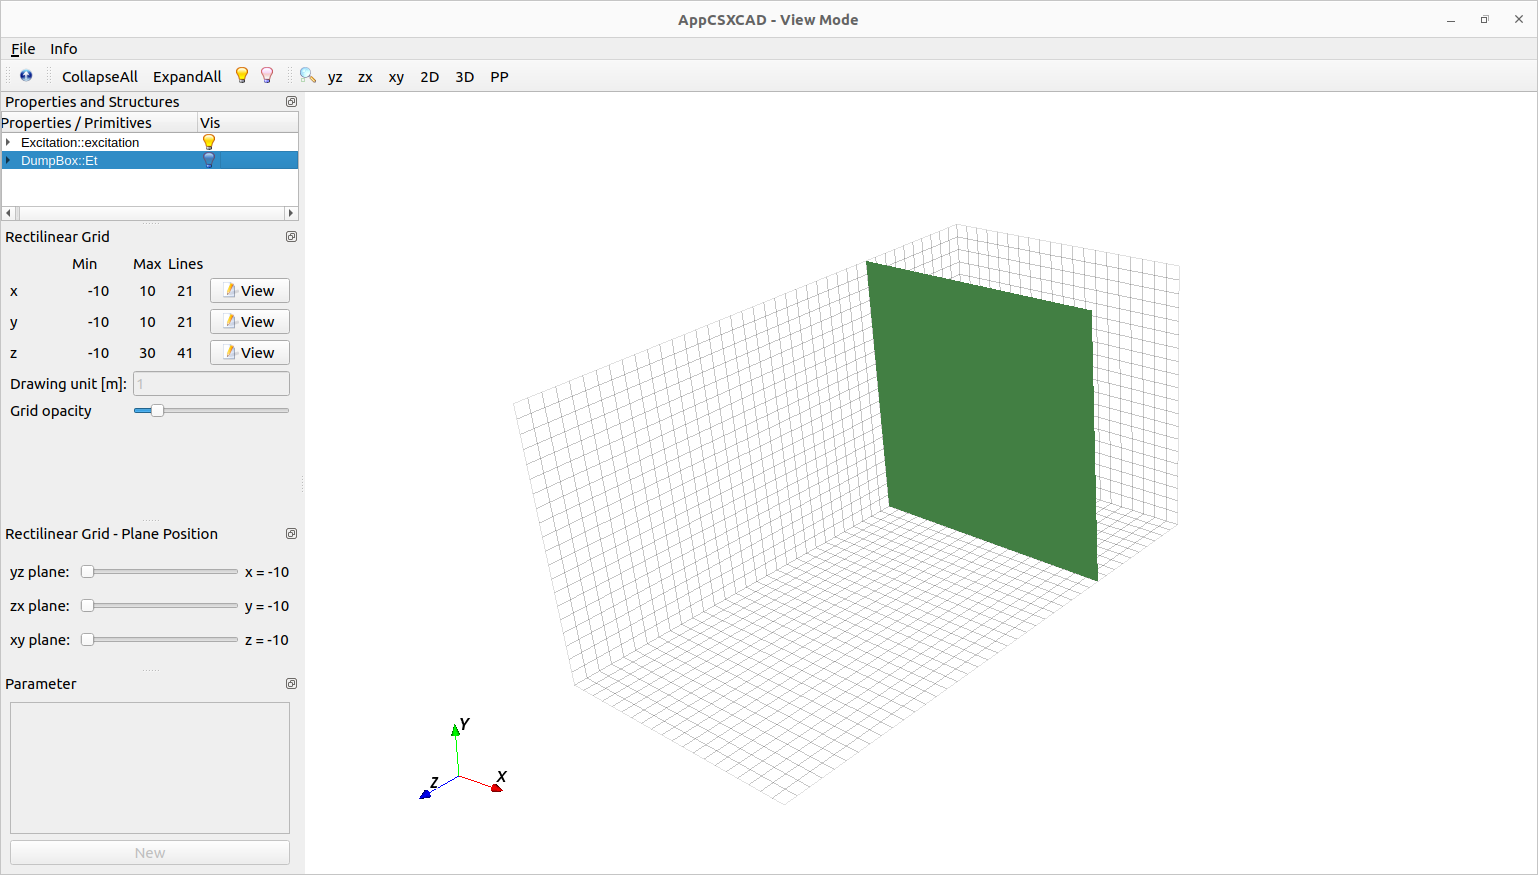
\includegraphics[width=\textwidth]{./img/geo1.png}
	\caption{Geometría del ejemplo 1.}
	\label{fig:geo1}
\end{figure}

Una vez satisfecho con la geometría, se procede a lanzar la simulación. Para
eso, primero debe cerrar el visualizador de geometría y escribir el siguiente
comando:

\begin{verbatim}
RunOpenEMS('tmp','tmp.xml','');
\end{verbatim}

Para visualizar la simulación se puede usar el programa ParaView. Para eso se
debe abrir el archivo \texttt{Et..vtr}, luego debe ingresar al inspector de
objetos y seleccionar que el color se asocie al \emph{E-Field} además de indicar
el eje \emph{Y}. Seguidamente,
puede hacer click en el boton de \emph{play}.
Se verá una animación con la variación del potencial eléctrico en el tiempo, sin
embargo los colores se encuentran sobre el plano y no se puede apreciar con
facilidad la onda.

Para mejorar la representación se debe colocar el filtro \emph{warp-by-vector}
que deformará la representación según la intensidad del campo, esto genera una
representación en donde se puede observar con facilidad la onda en la guía.

En la figura \ref{fig:sim1} se puede observar la guía de onda simulada en un plano.

\begin{figure}[htbp]
	\centering
	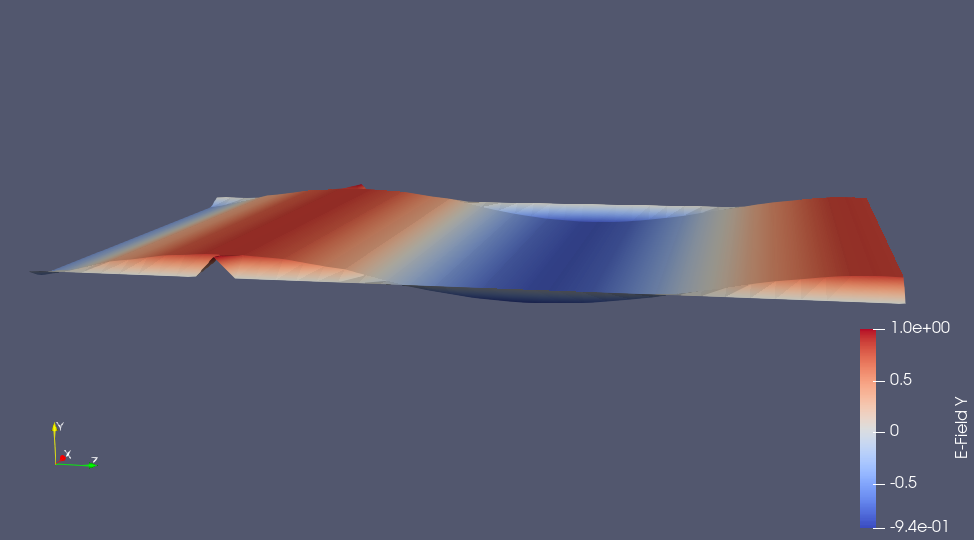
\includegraphics[width=\textwidth]{./img/sim1.png}
	\caption{Simulación del ejemplo 1.}
	\label{fig:sim1}
\end{figure}

\subsubsection{Esfera metálica dispersa un frente de onda}
\label{subsub:oejemplo2}

En este ejemplo se simula la dispersión que produce una esfera metálica cuando
una onda incide sobre ella.
Para tal fin se generó una geometría esférica con la propiedad física de ser un
conductor eléctrico. Se la puede ver en la figura \ref{fig:sim2}.

\begin{figure}[htbp]
	\centering
	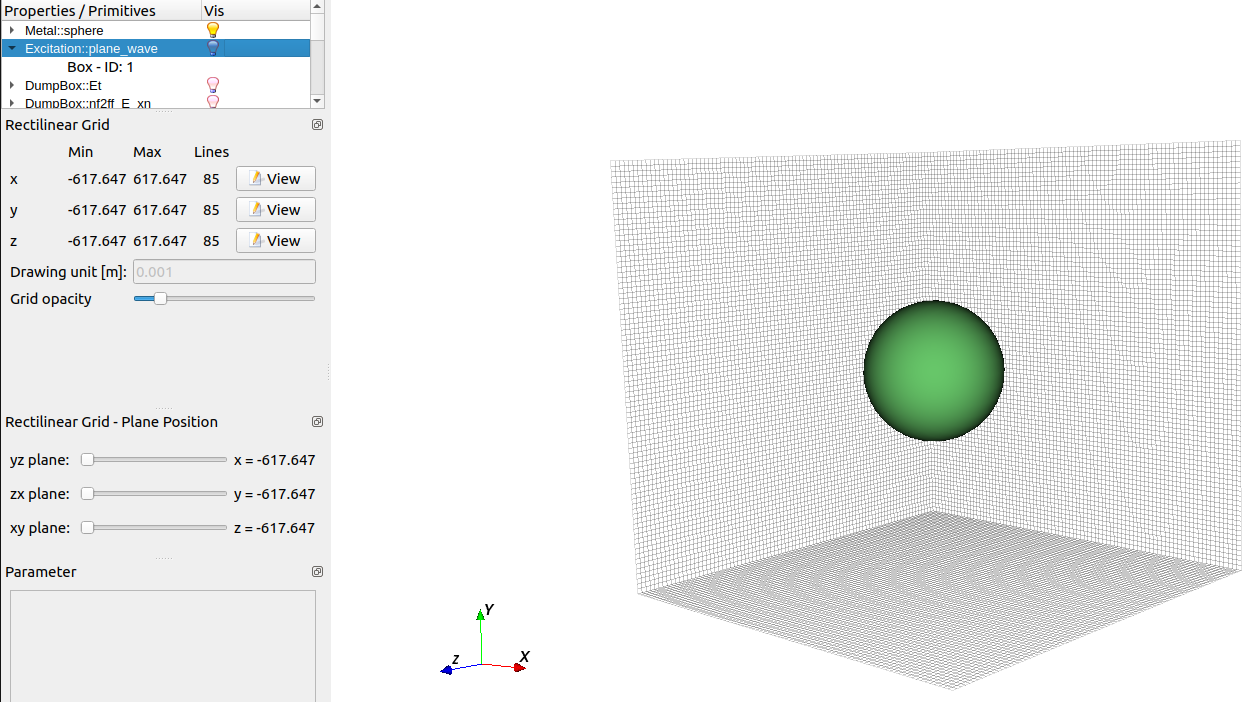
\includegraphics[width=\textwidth]{./img/ejemplo_esfera.png}
	\caption{Esfera metálica del ejemplo 2.}
	\label{fig:sim2}
\end{figure}

Luego se definió un cubo como volumen de simulación lo suficientemente grande
para que el cálculo numérico sea lo más preciso posible pero que los tiempos de
cómputo sean aceptables. El volumen se puede observar en la figura \ref{fig:sim3}.

\begin{figure}[htbp]
	\centering
	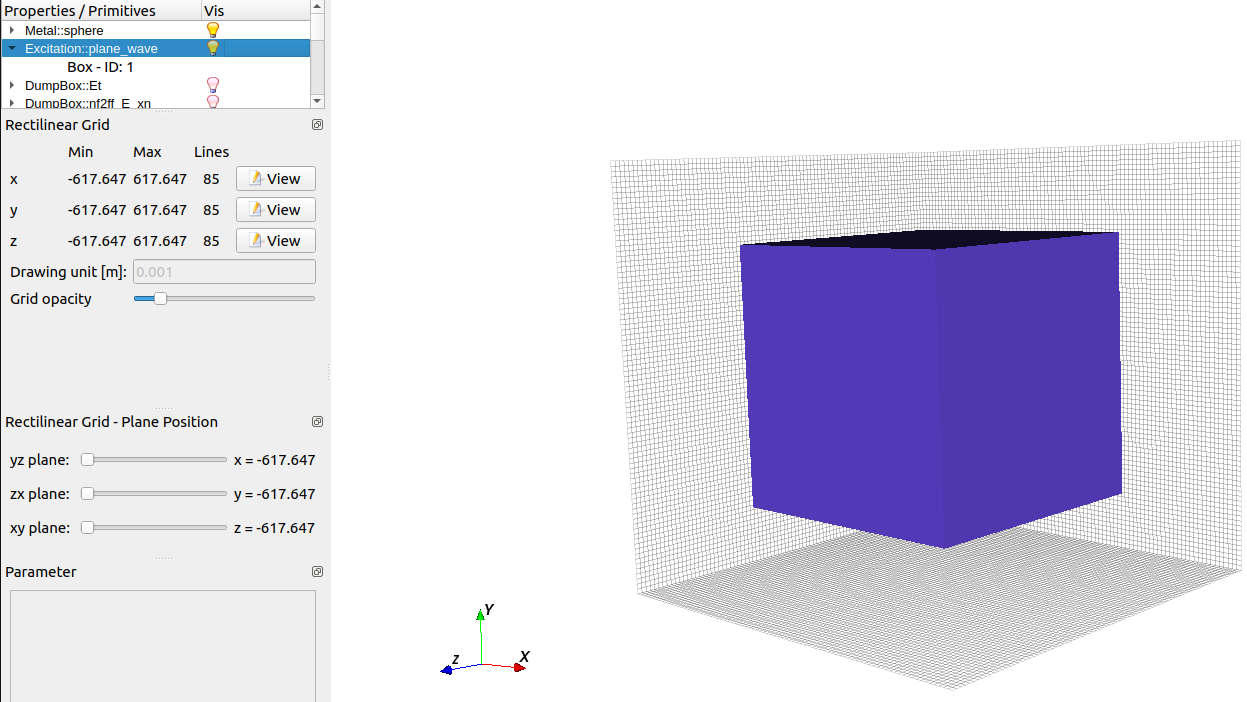
\includegraphics[width=\textwidth]{./img/ejemplo_cubo.png}
	\caption{Volumen de simulación del ejemplo 2.}
	\label{fig:sim3}
\end{figure}

Luego se corrió la simulación y se la visualizó con ParaView.
Se tomaron capturas en 3 momentos distintos y se los muestran en 2 y 3
dimensiones.
Se pueden observar en las figuras \ref{fig:sim4},\ref{fig:sim5},\ref{fig:sim6},\ref{fig:sim7},\ref{fig:sim8} y \ref{fig:sim9}.

A continuación se describe el código para generar el ejemplo:

\begin{verbatim}
% Si es la primera ejecución de octave de la sesión de trabajo
% agregar openEMS al path, sino physical_constants no va a estar
% definido
addpath('~/opt/openEMS/share/openEMS/matlab');
addpath('~/opt/openEMS/share/CSXCAD/matlab');

close all
clear
clc

%% Se configura la simulación
physical_constants;
unit = 1e-3; % longitudes en mm

sphere.rad = 200;

inc_angle = 0 /180*pi; % ángulo incidente (x-axis) en rad

% Tamaño de la caja de simulación
SimBox = 1000;
PW_Box = 750;

%% configuración FDTD parámetros y función de excitación
f_start =  50e6; % frecuencia de inicio
f_stop = 1000e6; % frecuencia de fin
f0 = 500e6;

FDTD = InitFDTD( );
FDTD = SetGaussExcite( FDTD, 0.5*(f_start+f_stop), 0.5*(f_stop-f_start) );
BC = [1 1 1 1 1 1]*3;  % set boundary conditions
FDTD = SetBoundaryCond( FDTD, BC );

%% configurar CSXCAD geometría y malla
max_res = c0 / f_stop / unit / 20; % cell size: lambda/20
CSX = InitCSX();

% creación de malla
smooth_mesh = SmoothMeshLines([0 SimBox/2], max_res);
mesh.x = unique([-smooth_mesh smooth_mesh]);
mesh.y = mesh.x;
mesh.z = mesh.x;

%% creación de esfera de metal
CSX = AddMetal( CSX, 'sphere' ); % se crea un conductor perfecto (PEC)
CSX = AddSphere(CSX,'sphere',10,[0 0 0],sphere.rad);

%% excitación de onda planar
k_dir = [cos(inc_angle) sin(inc_angle) 0]; % dirección de la onda planar
E_dir = [0 0 1]; % polarización de la onda planar --> E_z

CSX = AddPlaneWaveExcite(CSX, 'plane_wave', k_dir, E_dir, f0);
start = [-PW_Box/2 -PW_Box/2 -PW_Box/2];
stop  = -start;
CSX = AddBox(CSX, 'plane_wave', 0, start, stop);

CSX = AddDump(CSX, 'Et');
start = [mesh.x(1)   mesh.y(1)   0];
stop  = [mesh.x(end) mesh.y(end) 0];
CSX = AddBox(CSX, 'Et', 0, start, stop);

%% cálculo nf2ff
start = [mesh.x(1)     mesh.y(1)     mesh.z(1)];
stop  = [mesh.x(end) mesh.y(end) mesh.z(end)];
[CSX nf2ff] = CreateNF2FFBox(CSX, 'nf2ff', start, stop);

mesh = AddPML(mesh,8);

CSX = DefineRectGrid( CSX, unit, mesh );

%% carpeta de simulación
Sim_Path = 'Sphere_RCS';
Sim_CSX = 'Sphere_RCS.xml';

[status, message, messageid] = rmdir( Sim_Path, 's' );
[status, message, messageid] = mkdir( Sim_Path );

WriteOpenEMS( [Sim_Path '/' Sim_CSX], FDTD, CSX );

%% Se muestra la geometría
CSXGeomPlot( [Sim_Path '/' Sim_CSX] );

%% se corre la simulación
RunOpenEMS( Sim_Path, Sim_CSX);
\end{verbatim}
\begin{figure}[htbp]
	\centering
	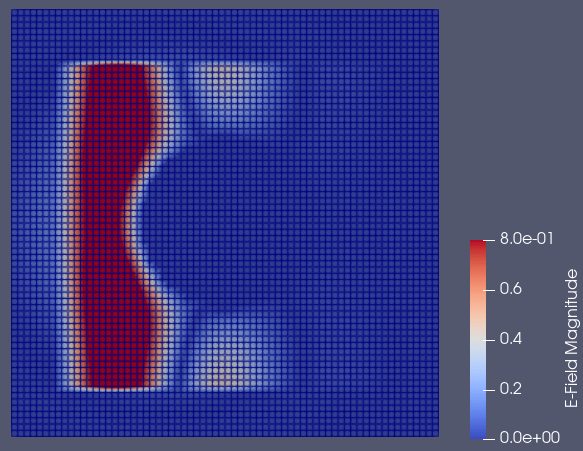
\includegraphics[width=\textwidth]{./img/impacto.png}
	\caption{Simulación momento 1.}
	\label{fig:sim4}
\end{figure}

\begin{figure}[htbp]
	\centering
	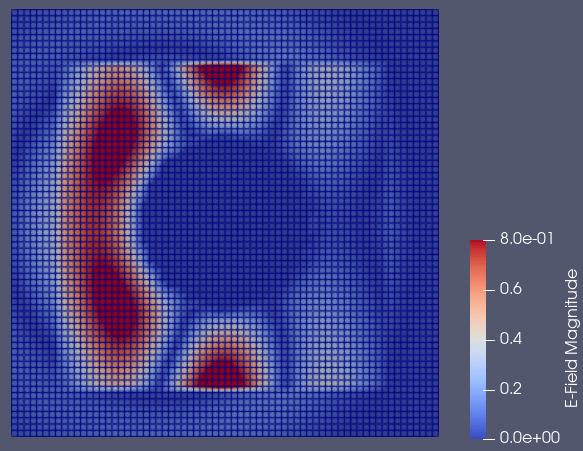
\includegraphics[width=\textwidth]{./img/mitad.png}
	\caption{Simulación momento 2.}
	\label{fig:sim5}
\end{figure}

\begin{figure}[htbp]
	\centering
	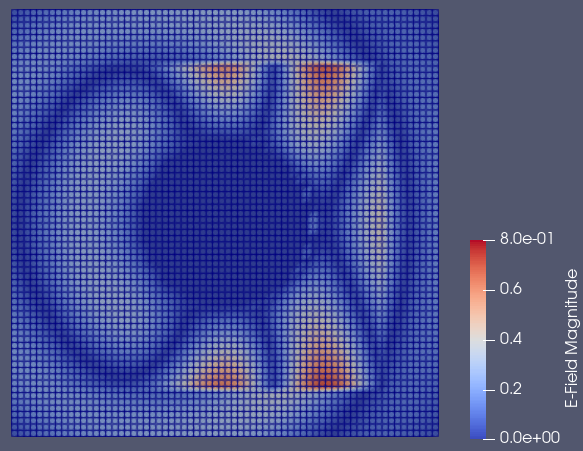
\includegraphics[width=\textwidth]{./img/salida.png}
	\caption{Simulación momento 3.}
	\label{fig:sim6}
\end{figure}

\begin{figure}[htbp]
	\centering
	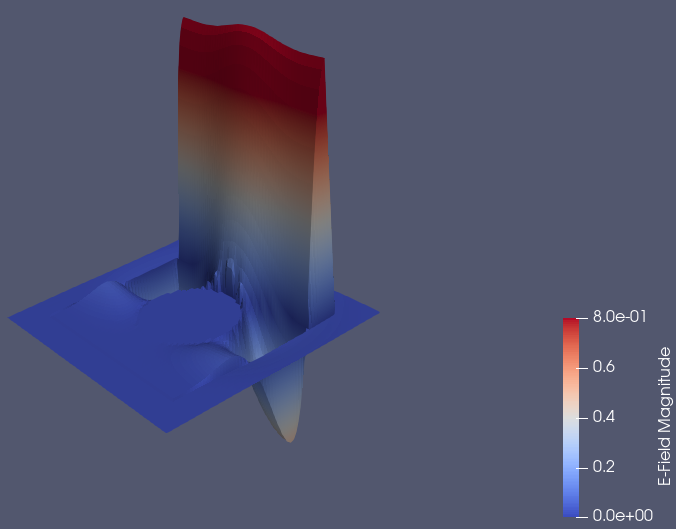
\includegraphics[width=\textwidth]{./img/impacto3d.png}
	\caption{Simulación momento 1 en 3D.}
	\label{fig:sim7}
\end{figure}

\begin{figure}[htbp]
	\centering
	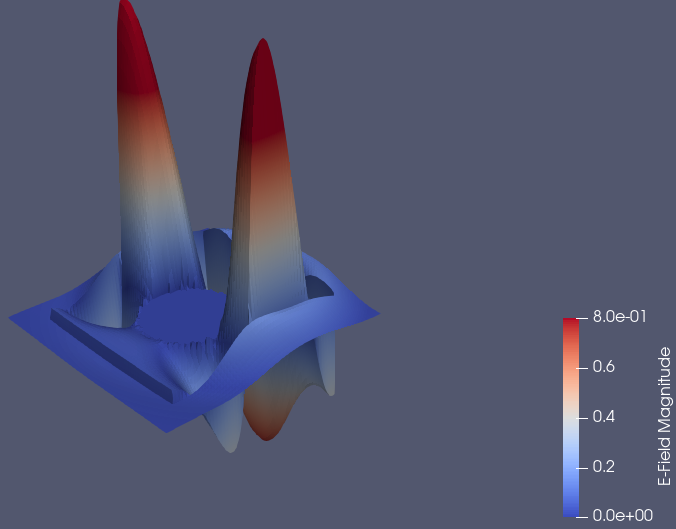
\includegraphics[width=\textwidth]{./img/mitad3d.png}
	\caption{Simulación momento 2 en 3D.}
	\label{fig:sim8}
\end{figure}

\begin{figure}[htbp]
	\centering
	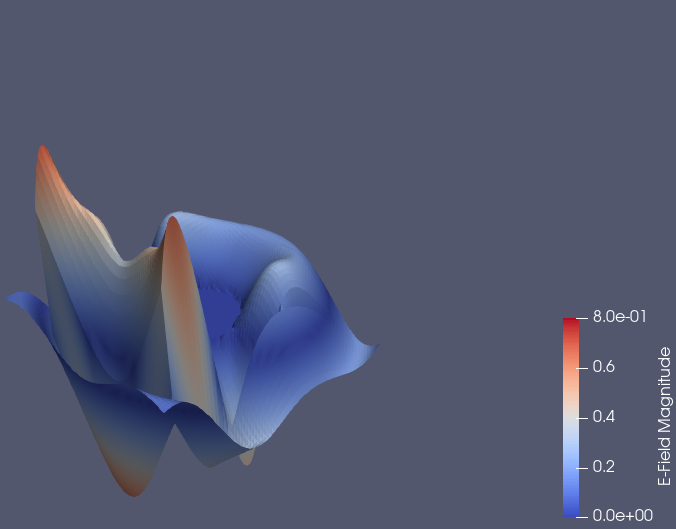
\includegraphics[width=\textwidth]{./img/salida3d.png}
	\caption{Simulación momento 3 en 3D.}
	\label{fig:sim9}
\end{figure}

\end{document}